\documentclass[compress]{beamer}
\usepackage{graphicx}
\usepackage{enumerate}
\usepackage{amssymb}
\usepackage{cancel}
\usepackage[utf8]{inputenc}
\usepackage[T1]{fontenc}
\usepackage{color}
\usepackage{array}
\usepackage{bytefield}
\newcolumntype{d}[1]{D{.}{.}{#1}}
\usepackage[francais]{babel}
\usepackage{tikz}
\usepackage{soul}
\usepackage{listings}
\newcommand{\esN}{\mathbb{N}}
\newcommand{\esR}{\mathbb{R}}
\usetheme[navigation]{UMONS}
\setbeamertemplate{caption}[numbered]
\title{EXIP, un framework de développement Web embarqué}
\date{10 nov. 2016}
\author[Z. \textsc{Bouali}, G. \textsc{Huysmans}]
	{Zakariae \textsc{Bouali}, Guillaume \textsc{Huysmans}}
\institute[]{Département d'Informatique \\
	Université de Mons \\[2ex]
\includegraphics[height=4ex]{UMONS}\hspace{2em}
	\raisebox{-1ex}{
\includegraphics[height=6ex]{UMONS_FS}}}
\bibliographystyle{plain}
\begin{document}
\begin{frame}
	\maketitle
\end{frame}
\begin{frame}
	\frametitle{Plan}
	\tableofcontents
\end{frame}


\section{Introduction}
\begin{frame}
	\frametitle{XML : eXtensible Markup Language}
	\begin{itemize}
	\item \href{https://www.w3.org/TR/xml/}{Standardisé}
		par le World Wide Web Consortium (W3C) \pause
	\item Format texte... \pause simple et lisible mais plus gourmand \pause
	\item Largement utilisé \pause (SVG, SOAP, RSS, ATOM, XHTML...) \pause
	\item Flexible \pause <<~mais pas trop non plus~>> (XML Schema) \pause
	\end{itemize}
	JSON, ASN.1... ne disposent pas d'un mapping formel entre elles et XML :
	moins d'interopérabilité avec les technologies Web.
\end{frame}
\begin{frame}
	\frametitle{Embedded Devices}
	\begin{itemize}
	\item Plus d'objets connectés que de citoyens américains en 2013 ! \pause
	\item Contraintes : \pause
		\begin{itemize}
		\item capacité mémoire \pause
		\item puissance de calcul \pause
		\item bande passante \pause
		\item réserve énergétique \pause
		\end{itemize}
	\item Besoin d'un protocole léger !
	\end{itemize}
\end{frame}

\section{EXI}
\begin{frame}
	\frametitle{EXI : Efficient XML Interchange}
	\begin{itemize}
	\item \href{https://www.w3.org/TR/exi/}{Standardisé}
		par le World Wide Web Consortium (W3C) \pause
	\item Format <<~binaire~>> car le texte est parfois redondant : \pause
		\begin{itemize}
		\item gain en bande passante et en stockage \pause
		\item traitement plus simple \pause
		\end{itemize}
	\item Séquence d'événements, grammaire régulière \pause
	\item Extension de la grammaire en cours d'exécution \pause
	\item XML Schema encodé de la même manière
	\end{itemize}
\end{frame}
\begin{frame}
	\frametitle{EXI Stream}
	\begin{itemize}
	\item \emph{Header} : la version, des paramètres d'encodage... \pause
	\item \emph{Body} : suite d'événements composés au plus de 3 naturels
		(séquences plus courtes si répétées, à la Huffman) suivis
		de leur contenu éventuel (nom et valeur d'un attribut, etc.) \pause
		\begin{itemize}
		\item \emph{SE} name, \emph{EE} : début \& fin d'élément \pause
		\item \emph{AT} name, value : attribut \pause
		\item \emph{CH} value : caractères \pause
		\item etc. \pause
		\end{itemize}
	\end{itemize}

	Le texte est stocké dans des tables (répétitions gratuites).
\end{frame}
\begin{frame}
	\frametitle{EXemple}
	\only<1>{
	\begin{figure}[h]
	\lstinputlisting[language=xml]{document.xml}
	%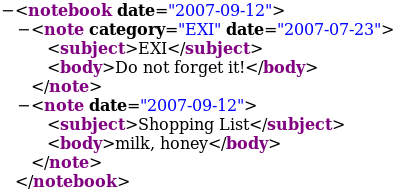
\includegraphics[width=\textwidth]{document.png}
	\caption{Document XML \cite{pei}}
	\end{figure}
	}
	\only<2>{
	\begin{figure}[h]
	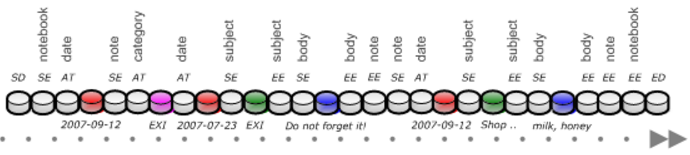
\includegraphics[width=\textwidth]{stream_zoom.png}
	\caption{\emph{EXI Body} correspondant \cite{pei}}
	\end{figure}
	}
\end{frame}
\begin{frame}[t]
	\frametitle{Grammaires}
	Une pile contient les grammaires en cours d'utilisation. \pause

	Elles correspondent chacune à une expression régulière
	\only<2>{et avec EXIP, après
	concaténation, restent régulières et non ambiguës (automate fini).

	On empile chaque règle exécutée et la dépile une fois \textit{matchée}.

	Un nom qui y apparaît est local, pas comme dans un DTD.
	\begin{figure}[h]
	NOTEBOOK $\rightarrow$ <notebook>.(NOTE)*.</notebook> \\
	NOTE $\rightarrow$ <note>.(SUBJECT)?.BODY.</note> \\
	SUBJECT $\rightarrow$ <subject>.[UTF-8 characters]*.</subject> \\
	BODY $\rightarrow$ <body>.[UTF-8 characters]*.</body>
	\caption{Extended Context-Free Grammar \cite{kyu}}
	\end{figure}
	}
	\only<3>{
	\begin{figure}[h]
	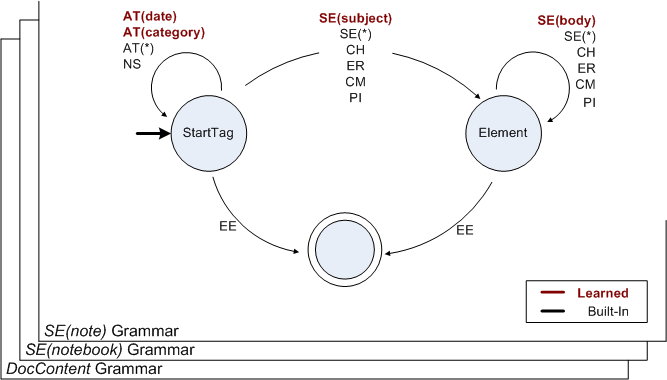
\includegraphics[width=.7\textwidth]{stack.png}
	\caption{Strict Schema-Informed Grammar for SE(note) \cite{pei}}
	\end{figure}
	}
\end{frame}
\begin{frame}
	\frametitle{Performances}
	\begin{figure}[h]
	%FIXME décodage plutôt ? plus parlant
	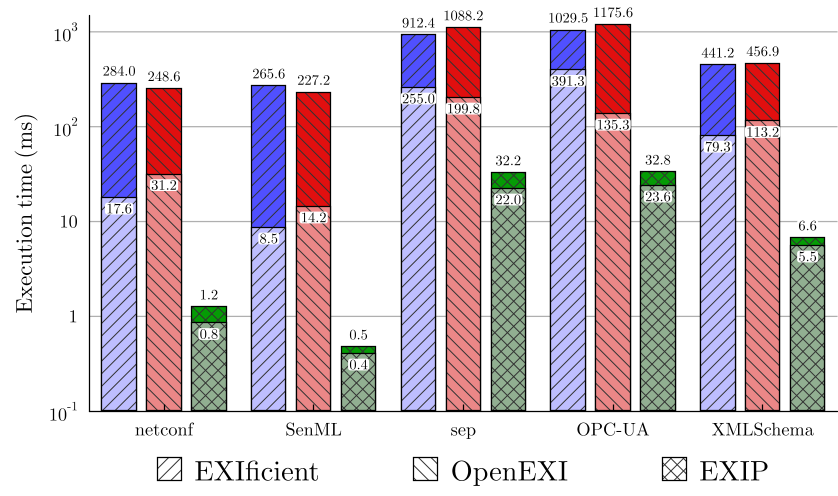
\includegraphics[width=.8\textwidth]{perfs.png}
	\caption{Temps de génération de la grammaire (échelle logarithmique).
		En foncé, temps gagné grâce aux optimisations. \cite{kyu}}
	\end{figure}
\end{frame}

\section{CoAP}
\begin{frame}
	\frametitle{Constrained Application Protocol (CoAP)}
	\begin{itemize}
		\item Protocole conçu par l'IETF : RFC 7252 \cite{rfc7252} \pause
	\item Orienté requête/réponse avec GET, POST, PUT, DELETE... \\
		REST\footnote{REpresentational State Transfer, <<~sans état~>>}ful \pause
	\item URIs\pause, \emph{Content-Type}\pause,
		mise en cache simple (\emph{max-age}) \pause
	\item \emph{Subscriptions, Push Notifications} \pause
	\item Mapping HTTP : proxy
	\end{itemize}
\end{frame}
\begin{frame}
	\frametitle{Protocol Stacks}
	\begin{table}[h]
	\center
	\begin{tabular}{l|l}
		HTTP & CoAP \\ \hline \pause
		TCP,
			UDP\footnote{SSDP utilise des messages ressemblant à du HTTP}
			& UDP \\ \hline \pause
		IP & 6LoWPAN \\ \hline \pause
		Ethernet, IEEE 802.11 & ContikiMAC, X-MAC \\ \hline \pause
		PHY & IEEE 802.15.4, Low-Power WiFi
	\end{tabular}
	\caption{Comparaison HTTP/CoAP}
	\end{table}
	\pause
	CoAP est <<~au total~>> plus facile et économique à traiter qu'HTTP
	qui nécessite entre autres une implémentation de TCP.

	Le contrôle de la couche transport est reporté au niveau
	applicatif (certains messages pourront ne pas être acquittés).
\end{frame}
\begin{frame}[fragile]
	\frametitle{CoAP Message}
	\begin{table}
	\begin{bytefield}[bitwidth=0.8em]{32}
	\bitheader{0-31} \\
	\begin{rightwordgroup}{UDP \\ Header}
	\bitbox{16}{Source Port} & \bitbox{16}{Destination Port} \\
	\bitbox{16}{Length} & \bitbox{16}{Internet Checksum}
	\end{rightwordgroup} \\
	\begin{rightwordgroup}{CoAP \\ Header}
	\bitbox{2}{Ver} & \bitbox{2}{T} & \bitbox{4}{TKL} &
	\bitbox{8}{Code} & \bitbox{16}{Message ID} \\
	\wordbox{1}{Token (if any, TKL bytes)} \\
	\wordbox{1}{Options (if any)}
	\end{rightwordgroup} \\
	\wordbox{3}{Payload (if any)}
	\end{bytefield}
	\caption{Message CoAP dans UDP, remis en forme à partir de \cite{rfc7252}}
	\end{table}
	T : \emph{Confirmable}, \emph{Non-Confirmable}\pause,
		\emph{ACK}\pause, \emph{Reset}...
\end{frame}
\begin{frame}
	\frametitle{CoAP Dialog}
		\center
	\begin{minipage}[b]{.6\textwidth}
	\begin{figure}[h]
	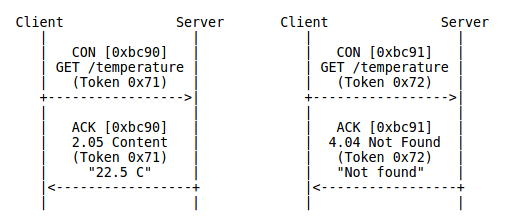
\includegraphics[width=\textwidth]{coap_normal.png}
	\caption{GET réussi/échoué \cite{rfc7252}}
	\end{figure}
	\end{minipage}
	\begin{minipage}[b]{.3\textwidth}
	\begin{figure}[h]
	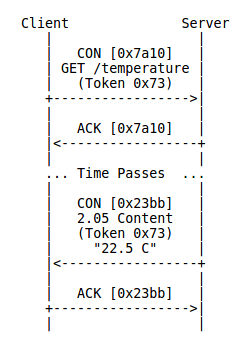
\includegraphics[width=\textwidth]{coap_push.png}
	\caption{Push Notification \cite{rfc7252}}
	\end{figure}
	\end{minipage}
\end{frame}
\begin{frame}
	\frametitle{Web Page Engine (XHTML/EXI)}
	\begin{figure}[h]
	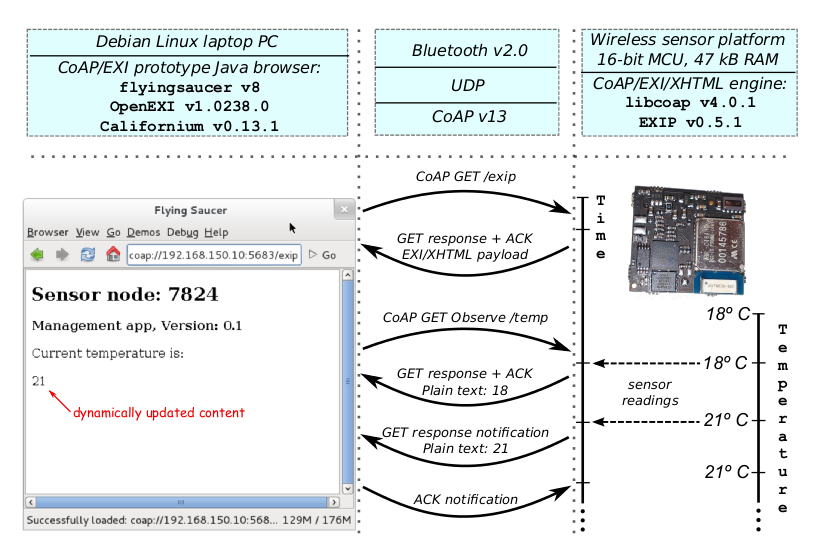
\includegraphics[width=.8\textwidth]{browser.png}
	\caption{Communication entre un navigateur en Java et
	un capteur sans fil \cite{kyu}}
	\end{figure}
\end{frame}
%FIXME perfs d'EXI

\section{Conclusion}
\begin{frame}
	\frametitle{Conclusion}
	Le Web n'est pas réservé aux périphériques puissants :
	\begin{itemize}
		\item XML n'est pas toujours synonyme de lourdeur !
		\item Il n'y a pas que HTTP/TCP dans la vie (et c'est standardisé)
	\end{itemize}
\end{frame}

\appendix
\begin{frame}
	\frametitle{Références}
	\bibliography{article}
\end{frame}

\begin{frame}[t]
	\frametitle{Questions ?}
	\center
	\vspace{-2em}
	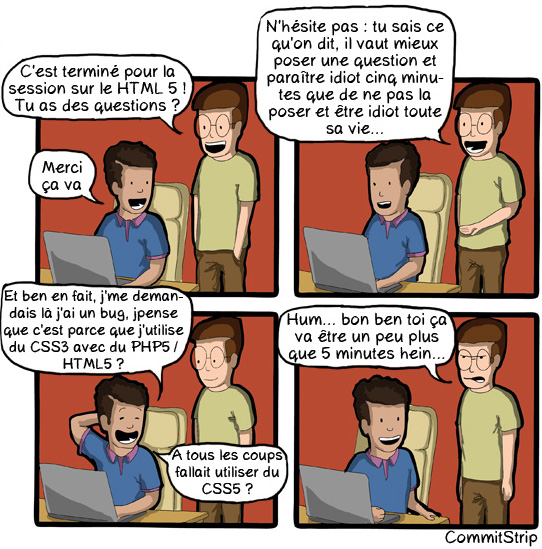
\includegraphics[width=.6\textwidth]{questions-html5_commitstrip.jpg}
\end{frame}
\end{document}
